%
% Sample SBC book chapter
%
% This is a public-domain file.
%
% Charset: ISO8859-1 (latin-1) áéíóúç
%
\documentclass{SBCbookchapter}
\usepackage[utf8]{inputenc}
\usepackage[T1]{fontenc}
\usepackage[brazilian,english]{babel}
\usepackage{graphicx}
\usepackage[pdftex]{hyperref} % para links e afins!
\usepackage{listings} % para utilização de código e highlight

\usepackage{listings-golang} % import this package after listings
\usepackage{color}
\lstset{ % add your own preferences
	basicstyle=\ttfamily,
	frame=l,
	keywordstyle=\color{red},
	numbers=left,
	numbersep=10pt,
	showstringspaces=false, 
	stringstyle=\color{blue},
	tabsize=4,
	language=Golang % this is it 
}


\author{Diego Fernando de Sousa Lima, Leonardo Augusto Gomes da Silva}
\title{Uma Introdução ao Go: A Linguagem Performática do Google}

\begin{document}
\maketitle

\begin{abstract}
	This meta-paper describes the style to be used in articles and short
	papers for SBC conferences. For papers in English, you should add just
	an abstract and for the papers in Portuguese, we also ask for an
	abstract in Portuguese (``resumo''). In both cases, abstracts should not
	have more than 10~lines and must be in the first page of the paper.
\end{abstract}

\begin{resumo}
	\begin{otherlanguage}{brazilian}
		Este meta-artigo descreve o estilo a ser usado na confecção de artigos
		e resumos de artigos para publicação nos anais das conferências
		organizadas pela SBC.  solicitada a escrita de resumo e abstract apenas
		para os artigos escritos em português. Artigos em inglês, deverão
		possuir apenas abstract. Nos dois casos, o autor deve tomar cuidado para
		que o resumo (e o abstract) não ultrapassem 10~linhas cada, sendo que
		ambos devem estar na primeira página do artigo.
	\end{otherlanguage}
\end{resumo}

\section{Introdução}

Ao longo do tempo, o desenvolvimento de \textit{software} foi se aprimorando e as ferramentas utilizadas para sua composição evoluindo de acordo com as necessidades que a tecnologia tende a resolver. Podemos então classificar as Linguagens de Programação como principal artefato deste meio por ser o intermédio onde computador processa informações afim de gerar saídas para o uso benéfico.

O ato de criar um novo \textit{software} pode requerer paciência, atenção e proatividade por parte do desenvolvedor e devido a isso as Linguagens de Programação estão sempre se renovando buscando maior proximidade com o programador e se tornando mais portáveis. O maior exemplo disso são as linguagens rotuladas como de alto nível nas quais podemos citar Python, PHP, Ruby, C++, Java, entre outras.

As linguagens de alto nível tem como característica principal o poder elevado de abstração aproximando o sintaxe à linguagem humana, diferentemente das linguagens de baixo nível, que por sua vez se assemelham ao código utilizado por máquina. Golang, como também é abreviada, fica entre as linguagens de alto nível, assim como colabora para facilitar o desenvolvimento sem perder o alto desempenho. A quantificação de seu desempenho é notado pelo poder de execução de suas \textit{threads}, veremos isso ao decorrer deste capítulo. 

As próximas seções deste capítulo detalham a linguagem desde seus conceitos principais, passando pela instalação e preparação do ambiente, sintaxe básica ponderando os elementos exclusivos da linguagem, e ao fim estão apresentados os módulos de programação para Web com Go com foco principal na construção de uma Rest API com a biblioteca nativa \texttt{http/net}.

\subsection{Porque Go}

A grande problematica do tempo long de compilação recorrente na maioria das linguagens usadas foi um dos principais motivos para a criação de Golang. Os grandes servidores da Google necessitavam de um grande poder de eficiencia e produtividade, para tornar aplicações escalaveis e mais rapidas. Em novembro de 2009 se deu inicio ao nascimento da limguagem performatica Golang dentro das dependencias dos escritorios da Google. Seu projeto de criação foi liderado por Rob Pike, Ken Thompson e Robert Griessemer.

Suas principais vantagens é seu poder de processamento que permite aplicações traalharem aproveitando o máximo do poder dos processadores multi-core de forma mais otimizada. Além de ser baseda em C com caracteristicas de tipagem forte e estática, alto nivel, Structs e garbage collection. Tal poder de processamento é oriundo das "goroutines" que são rotinas de leves que se comunicam por channels, evitando o uso de memória compartilhada evitando tecnicas de sincronizações mais pesadas como "semáforos".


O Go embora sejá recente ela dá suporte a varias bibliotecas para a criação de ferramentas de comunicação em rede, servidores HTTP, expressões regulares, leitura e escrita de arquivos. Por ser robusta ela exige um certo nível de atenção na sua codificação, porém isso torna-se uma vantegem por doutrinar os codificadores a produzirem códigos mais limpos e padronizados. No mercado atual Go já possui seu espaço, principalmente como uma possível sucessora da linguagem C, por suportar a demanda de trabalho em servidores e sistemas multi-thread. Além de ser uma mais usadas e divulgada pela Google, expandindo-se ainda mais pela a força do nome de uma das maiores empresas multinacional do mundo. 

\subsection{Go atualmente}

Devido seu diferencial, Golang está em plena ascenção. O reflexo de seu crescimento é representado pela sua utilização nos dias atuais, tanto por empresas internacionais como nacionais. Além da própria Google, outras companhias usam Go em suas infraestruturas, é possível citar: Adobe, BBC, Canonical, Dell, DigitalOcean, Dropbox, Facebook, IBM, Mozilla, SoundCloud, Twitter, Yahoo, entre outras.

No Brasil não é diferente, muitas companhias estão aderindo ao Go. Entre as empresas e instituições com maior respaldo estão: Globo.com, Magazine Luiza, Mercado Livre, Dafiti, PagSeguro, Pagar.me, Jusbrasil, Hotel Urbano, Walmart, Nuveo, Nic.br, entre outras. A lista completa de companhias que usam Go pelo mundo está no repositório oficial da linguagem no GitHub\footnote{\url{https://github.com/golang/go/wiki/GoUsers}}.

\section{Instalando e configurando o Go}

Neste topico estão disponiveis os passos para a instalação em dois SO's (Windows e Linux (Baseado em Debian)) dinstintos todos com suporte a instalação da linguagem Go em seu links ofciais que pussuem instruções faceis para seu uso desde a instalação de pacotes a configuração de variaveis de ambiente.

\subsection{Windows}

O Go pode ser instalado de duas formas no Windows, mas vamos aqui descrever a forma mais coniavel e recomendavel: que pode ser feito pelo instalador de automático que esta disponivel nesse link \url{https://golang.org/doc/install?download=go1.9.1.windows-amd64.msi}.  Apos feito o download o executavel por padão é salvo na pasta de download do seu computador em \texttt{C:\char`\\Dowloads\char`\\}.

Para que ele possa fazer a instalação dos pacotes necessarios para a linguagem basta clicar com o botão direito do mouse no executavel e com o botão esquerdo clicar em instalar. os binarios serão descarregados direto no seu disco disco local principal com o caminho \texttt{C:\char`\\Go}.

\begin{figure}[h]
	\centering
	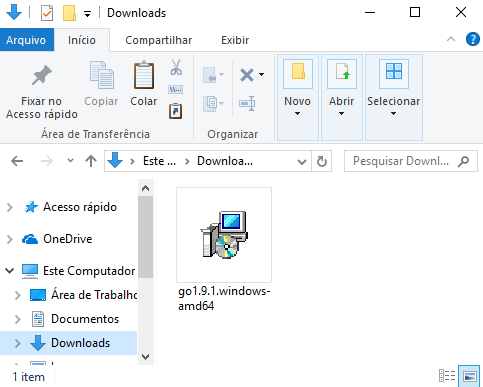
\includegraphics[width=0.5\linewidth]{diretorio.png}
	\caption{Executavel no Windows}
	\label{fig:gf}
\end{figure}

O seguinte passo será a configuração da variavel ambiente para a chamada do compilador instalado no seu computador. Para isso faz-se necessario que sejá configurado o caminho correto no seu sistema. Basta clicar como botão direito do mouse em seu diretorio principal da sua maquina, apos isso clique em propiedades. Fazendo esse passos aparecera as configurações de sistema, clicando em configurações avançadas aparecera uma nova janela em que uma das opções está as variaveis de ambiente e clique novamente:

\begin{figure}[h]
	\centering
	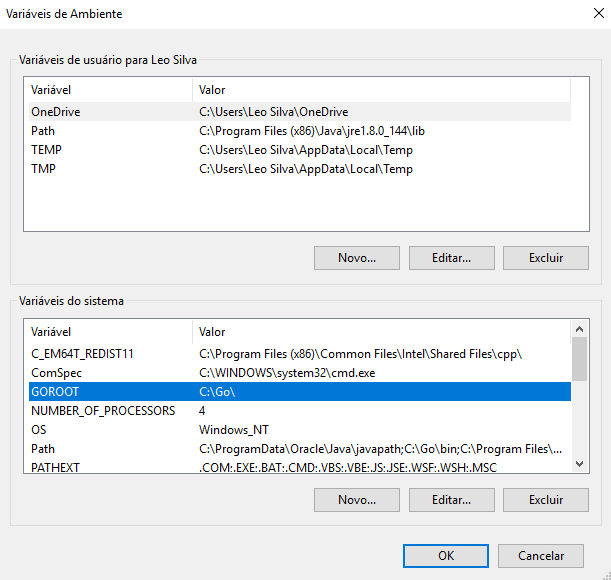
\includegraphics[width=0.5\linewidth]{ambiente.png}
	\caption{Variavel Ambiente no Windows}
	\label{fig:gf}
\end{figure}

Para finalizar todo o processo de configuração da variavel você deve indicar o caminho especifico de onde foi instalado. Para isso deve-se escrever o caminho \texttt{C:\char`\\Go;}. É importante por o ponto e virgula no final para indicar aonde deve ser parado a busca do ser complidador do linguagem, isso podera evitar alguns erros de execução em relação ao tempo. por ultimo basta abrir seu prompt de comando e digitar:


\texttt{C:\char`\\>go version} e clicar entre para aparecer a seguinte resposta: \texttt{go version go1.3 windows/amd64}, isto é a versão do seu Go. 
\subsection{Linux}

\section{Estrutura básica e sintaxe}

Após a instalação e configuração, você já pode criar seus primeiros programas. Esta seção é composta por elementos que constituem a sintaxe básica de Go. Programas em Go podem ser desenvolvidos em qualquer editor de texto que dê suporte a codificação \texttt{UTF-8}. Todos os exemplos mostrados nas próximas seções tem foco na execução em ambiente Linux baseado em Debian.

\subsection{Hello World}

Para primeiro contato com a linguagem, podemos iniciar com um tradicional \textit{Hello, World}. Portanto, salve um arquivo com título de sua preferência (sugerimos \texttt{hello.go}) e com o seguinte conteúdo:

\begin{lstlisting}
package main

import "fmt"

func main() {
	fmt.Println("Hello World!")
}
\end{lstlisting}

Para executar o código acima, basta ir na pasta do \texttt{GOPATH} (\texttt{\$GOPATH/src}) e execute \texttt{\$ go run hello.go}. A saída para este programa será:

\texttt{\$ Hello World}

Neste primeiro exemplo pode-se notar algumas caraterísticas, a primeira delas é que Go não possui ponto-e-vírgula (\texttt{;}) ou quaisquer ponto ou acentuações ao final das instruções, diferentemente de linguagens como C ou Java. Todo código em Go é dividido em três seções principais: 

\begin{enumerate}
	\item \textbf{Declaração do pacote}: Todo arquivo Go tanto deve existir dentro de um pacote, como deve ter um pacote chamado \texttt{main} com a função main (\texttt{func main()});
	\item \textbf{Declaração de dependências}: A segunda seção é destinada as dependências externas de um programa em Go, podendo elas serem opcionais. No nosso exemplo, usamos o \texttt{fmt} para auxiliar na entrada e saída de dados pelo terminal;
	\item \textbf{Código}: Por último, temos o código de fato. Nele é onde aplicamos a lógica e é a parte central de um programa em Go.
\end{enumerate}

A função \texttt{main} de um programa em Go não recebe parâmetros, nem retorna valores. Mais uma característica que a difere de linguagens como o Java ou C.
Para comando de entrada e saída, podemos usar as funções provenientes do pacote \texttt{fmt}. O \texttt{fmt.Println()} imprime o conteúdo seguido de quebra de linha, enquanto que \texttt{fmt.Print()} imprime apenas o conteúdo. Abordamos isso melhor na seção \ref{secaodeio}.

\subsection{Variáveis}

Go tem tipagem forte e estática, isso quer dizer que o tipo das variáveis declaradas durante a execução de um programa não podem ser alterado. Apesar deste conjunto de características, Go traz em sua sintaxe uma forma de declaração limpa, o que facilita e se torna eficiente na rapidez para o desenvolvimento das aplicações.

Além disso, o Go também faz abstrações do tipo \textit{Duck Tipyng} baseadas em \textit{interfaces} que é abordado na seção \ref{duck}.

A declaração de variáveis em Go pode ser de duas maneiras principais:

\begin{lstlisting}
package main

import "fmt"

func main() {
	var variavel_a int // tipo 1
	variavel_b := 5 // tipo 2
	
	var variavel_c int = 45 // tipo 3
	var x, y int = 1, 2 //tipo 4
}
\end{lstlisting}

O \textit{tipo 1} é usado quando não se sabe qual valor será alocado para a variável, enquanto o \textit{tipo 2} é uma maneira mais sucinta exclusiva do Go que força o tipo da variável de acordo com o valor recebido (note que o tipo não foi declarado). É importante considerar que o compilador só obtem sucesso em sua execução quando todas as variáveis instanciadas são devidamente usadas. Outros tipos de declaração são os tipos 3 e 4. Entre os tipos de variáveis suportados por Go estão \textbf{\textit{bool}}, \textbf{\textit{int}} \textit{(8, 16, 32, 64)}, \textbf{\textit{float}} \textit{(32, 64)}, \textbf{\textit{string}}, \textbf{\textit{byte}}, \textbf{\textit{rune}} e \textbf{\textit{complex}} \textit{(64, 128)}.

\subsubsection{Entrada e saída com fmt}
\label{secaodeio}

Com o pacote \texttt{fmt} é possível interagir com o usuário em modo texto no estilo \textit{input/output}. As funções principais de \texttt{fmt} tem função de entrada e saída de valores. O código abaixo mostram as funções de saídas mais comuns:

\begin{lstlisting}
package main

import "fmt"

func main() {
	str := "Gopher"
	
	fmt.Print("Ola ", str, "\n")
	fmt.Println("Ola", str)
	fmt.Printf("Ola %s\n", str)
}
\end{lstlisting}

As variações da função de impressão acima exibem a mesma saída:

\noindent\texttt{Ola Gopher}\\
\texttt{Ola Gopher}\\
\texttt{Ola Gopher}\\

Para receber uma entrada podemos usar a funcão \texttt{Scan} do pacote \texttt{fmt}. para fazer a leitura para uma variável, basta colocar a variável precedida do caractere \& entre os parênteses de \texttt{Scan}. Como exemplo:

\noindent\texttt{fmt.Scan(\&variavel)}\\

\subsection{Estrutura de seleção if/else}

A estrutura de seleção \texttt{if} tem a função básica de tomar decisões perante a execução de um programa. Em Go este tipo de estrutura difere em relação a outras linguagens, ela só recebe valores lógicos verdadeiro ou falso. Isso influencia definitivamete a tipagem da variavel que o comando vai receber, ou seja, as expressões necessitam ser do tipo \texttt{bool} e podem ser criadas funções ou métodos com a regra que todos retornem pelo menos um valor do tipo \texttt{bool}.

\begin{lstlisting}
idade := 22

if idade <= 18 {
	fmt.Println("Menor ou igual a 18 anos")
} else if idade > 25 {
	fmt.Println("Maior que 20 anos")
} else {
	fmt.Println("Entre 19 e 25 anos")
}
\end{lstlisting}

\subsection{Switch case}

A estrutura \texttt{switch case} tem funcionalidade parecida com o \texttt{if/else} visto na seção anterior. Dependendo do caso, o \texttt{switch case} pode se adequar melhor ao programa, especialmente em casos de Menus e estruturas de decisões com muitos opções. O \texttt{switch case} é orientado a casos tendo o caso \textit{default} escolhido quando nenhum dos outros forem satisfeitos. A sintaxe do \texttt{switch case} segue o seguinte modelo:

\begin{lstlisting}
t := time.Now()
switch {
case t.Hour() < 12:
	fmt.Println("Bom dia!")
case t.Hour() < 17:
	fmt.Println("Boa tarde.")
default:
	fmt.Println("Boa noite.")
}
\end{lstlisting}

\section{Coleções de dados}

Coleções de dados são tipos de variáveis especiais que podem serem entendidas como um conjunto ou listas de outras variaveis ou valores. Assim como em outras linguagens (ex: linguagem C com seus vetores) as coleções de dados são geralmente uma seguencia de valores encadeados em ordem predefinida ou até mesmo apenas espaços sepados não alocados para que depois venham ser preenchidos.


Em Go os padrões para listas de dados são dois: \texttt{arrays} e \texttt{slices}, o grande diferença entre os dois está relacionados a o espaço de alocação de mémoria. Os \texttt{arrays} são instacias com tamanho fixo, já os slices são uma camada abstratica dos arrays que podem ter sua alocação dinâmica podendo crescer de forma indefinida dando maior flexibilidade.

\subsection{Arrays}

Os Arrays são listas com valores do mesmo tipo, sendo que cada valor possui um indices que indica a posição dentro da lista, a contagem dos indices são delimitados pelo tamamaho do array que deve ser fixo e invariável. \textbf{Obs}: O primeiro elemento do array possui índice 0, e o último elemento é sempre \texttt{len(array) - 1}.


Podemos declarar um array em Go utilizando as seguintes formas:

\begin{lstlisting}
var colecao [3]int
pares := [3]int{2,4,6}
impares := [...]int{3, 5, 7}
nomes := [2]string{}

fmt.Println(colecao, pares, impares, nomes)

//Output: [0 0 0] [2 4 6] [3 5 7] [ ]
\end{lstlisting}

O tamanho do array sempres deve ser especificado na sua declaração, como por exemplo o array \texttt{colecao} que foi fixado em \texttt{[3]int}, ou seja , seu tamanho é de 3 posições inteiras. Podemos notar que ele a saida foi \texttt{[0 0 0]}, isso ocorre por que em Go quando se é declarado um array sua possições se não forem alocada ganham automaticamete valor \textit{zero value}.

Para vetores de outra tipagem esse valor atribuído automaticamente pode pode ser gerado de outras formas, vejamos a seguir:

\begin{itemize}
	\item \texttt{bool}: \texttt{false}, valor booleano falso;
	\item \texttt{int}: \texttt{0} , \textit{zero value};
	\item \texttt{float}: \texttt{0.0}, \textit{zero value} com ponto flutuante;
	\item \texttt{strings}: \texttt{""}, string vazia;
	\item \texttt{ponteiros}, \texttt{funções}, \texttt{interfaces}, \texttt{slices}, \texttt{maps} e \texttt{channels}: \texttt{nil}, valor nulo.
\end{itemize}


Há possibilidade de criar arrays multidimensionais em que os valores são arrays dentro de arrays. Declaramos eles da seguinte forma:


\begin{lstlisting}
var matrixA [2][2]int
matrixA[0][0], multiA[0][1] = 2, 8
matrixA[1][0], multiA[1][1] = 12, -1
matrixB := [2][2]int{{7, 23}, {-3, 10}}

fmt.Println("Matrix A:", matrixA)
fmt.Println("Matrix B:", matrixB)

//Output: Multi A: [[2 8] [12 -1]]
//Output: Multi B: [[7 23] [-3 10]]
\end{lstlisting}

Como já foi falado os arrays não são tão flexiveis como os slices que serão explicados no proxímo topico. Porém eles em sua importância dentro da linguagem Go. Cabe ressaltar que é possivel trabalhar com os array de for que eles venhm ficar dinamicos, mas requer um exforço manual custoso demais tendo que verificar seus limites, criação de arrays de cópias de valores, isso deixara o programa mais lendo e poluído.

\subsection{Slices}

Os slices são uma abstração que se basea em arrays que possibilitam mais flexibilidade na coleção de dados encadeados. Seu tamanho pode se espandir sem limites de tamanho, para declarar uma slice você ultiliza a mesma sintaxe de um array com a simples diferença de que não especificamos o tamanho. Vejamos a seguir exemplos aonde pode-se notar a semelhança:


\begin{lstlisting}
var lista []int
pares := []int{2, 4, 6}
nome := []string{}

fmt.Println(a, pares, nome)

//Output: [] [2 4 6] []
\end{lstlisting}

É possivel criar uma slice com a função \texttt{make}, que separa internamente um espaço de mémoria para um array retornando uma referência para o slice. Sua sintaxe pode ser escrita da seguibte forma:

\begin{lstlisting}
func make([]L, len, cap) []L

lista := make([]int, 10)
fmt.Println(lista, len(lista), cap(lista))

//Output: [0 0 0 0 0 0 0 0 0 0] 10 10

\end{lstlisting}

\texttt{L} indica o tipo de elementos que do \texttt{slice}, \texttt{len} o tamanho incial e \texttt{cap} a capacidade total de mémoria reservada. No slice lista é possivel analisar a saída em tres valores, o primeiro indica os elementos alocados (por padrão foi alocado o \textit{zero value}), o segundo esta a capacidade inicial 10 e por terceiro a final que também é 10.  

\subsection{Maps}

Os maps são uma estrutura de conjundo de dados se se organizão em \textbf{chave-valor}. em outras linguagens como Ruby e Python elas se assemelham há \textit{Hash} e \textit{Dictionary} respectivamente. Em Go elas são chamada também comohashtable, podemos associar essa estrutura também a tabelas em um banco de dados estruturado como \textit{MySQl}. Para se declarar um mapas em Go usamos a função \texttt{make()} ou a forma lideral, de forma que ser muito parecido com \texttt{slices}. No exemplo a seguir vamos declarar um mapa com chaves do tipo \texttt{int} sendo e valores \texttt{strings} sendo ele um mapa vazio:

\begin{lstlisting}
M1 := map[int]string{}
M2 := make(map[int]string)
\end{lstlisting}

Automaticamente os maps tem tamanho indefinido podendo ser alocado a quantidade de espaçoes necessarios possiveis durante a execução do programa tornando mais eficiente a facilidade de se trabalhar com dados diferentes sem a necessidade de saber tamanhos predefinidos aumentando a performace e evitando problemas de alocação. Recomenda-se sempre que for feita uma nova especificão de mémoria passando um segundo argumento à função \texttt{make()}:   

\begin{lstlisting}
M3 := make(map[int]string, 2066)
\end{lstlisting}
As formas literais de "popular" um mapa no momento da declaração e/ou atribuindo valores individualmente após a declaração:


\begin{lstlisting}
capitais := map[string]string{
	"GO": "Goiania",
	"PB": "Joao Pessoa",
	"PR": "Teresina"}

capitais["PR"] = "Curitiba"

fmt.Println(capitais)

//Output: map[GO:Goiania PB:Joao Pessoa PR:Curitiba]

\end{lstlisting}

Podemos notar que na primeira indicação da chave \texttt{"PR"} o valor especificado foi Teresina, e logo apos foi escrito o seguinte codigo: \texttt{capitais["PR"] = "Curitiba"}, ele permite que os valores sejam atualizados diretamente no em uma chave especifica de um map. Logo após a saída o valor que antes era Teresina foi trocado por \texttt{"Curitiba"}.
\subsection{Loops}

A estrutura basica de repetição em Go e o comando for, usado para fazer iterações com listas, slice, maps. Em sua forma mais comum é especificado uma condições lógica e o bloco código se repetirar até que a condição sejá satisfeita com verdadeiro:


\begin{lstlisting}
valor1, valor2 := 0, 20
for valor1 < valor2 {
valor1 += 1
}
\end{lstlisting}

O código que está assima será repetido em 20 iterações, ou seja, a variavel valor1 que recebe 0 na primeira linha sera incrementado com mais um até que ele satisfaça a condição do for do valor1 ser menor que o valor2 satisfazendo a condição de verdadeiro para a parada do comando.

Há a possibilidade de fazer iterações de forma tradicional parecidas com a linguagem C: 

\begin{lstlisting}
for i := 0; i < 10; i++ {
// ...
}
\end{lstlisting}

Assim como no exemplo anterior esse codigo executa qualquer bloco de codigo até que a condição de verdadeiro seja satisfeita, então o comando fará 10 iterações. Outra forma de fazer um iteração com for é feita sobre slices com auxilio do comando range:

\begin{lstlisting}
for indice, valor := range slice {
// ...
}
\end{lstlisting}

No codigo acima é retornado o índice de cada elemento do slice, para modificar valores desses slice podemos utilizar os índices. Assim basta somente omitir o segundo valor na atribuição e acessar cada elemento
através de seu índice: 


\begin{lstlisting}
numeros := []int{1, 2, 3, 4, 5}
for i := range numeros {
numeros[i] *= 2
}
fmt.Println(numeros)
//Output: [2 4 6 8 10]
\end{lstlisting}

Como ultimo exmplo podemos usar o for como um loop infinito como o while em outras linguegens:
\begin{lstlisting}
for {
// loop infinito
}
\end{lstlisting}
Para a padara do loop basta instanciar algum conmando de seleção como o if com o \texttt{break} interno.

\section{Funções}

Um dos pontos fortes da linguagem Go é a forma de variedades nas quais podemos escrever funções. Go permite que suas funções possam receber parâmetros, assim como também retornar valores podendo ser múltiplos. Até este momento neste capítulo usamos funções, pois a rotina de um código em Go deve iniciar da função \texttt{main()}. Nas seções seguintes detalhamos alguns dos tipos mais usados.

\subsection{Funções básicas}

Em Go o padrão básico de declaração das funções se dão com a palavra \texttt{func} seguido do nome da função e dos possíveis valores de parâmetros. Um exemplo seria uma função que imprima uma simples frase:

\begin{lstlisting}
func imprimirString() {
	fmt.Println("Imprimindo uma frase")
}
\end{lstlisting}

Agora iremos passar alguns argumentos para esta função, fazendo que ela imprima um valor do tipo \texttt{string} e outro do tipo \texttt{int}:

\begin{lstlisting}
func imprimirString(nome string, idade int) {
	fmt.Printf("Ola, meu nome eh %s e eu tenho %d anos.\n",
	nome, idade)
}
\end{lstlisting}

Caso os argumentos passados para a função sejam do mesmo tipo, é possível agrupá-los em uma única especificação:

\begin{lstlisting}
func intervalo(x, y int) {
	for i := x; i < y; i++ {
		fmt.Printf("%d ", i)
	}
}
\end{lstlisting}

Para retornar valores em uma função é necessário definir seu tipo logo após a passagem de parâmetros. Além disso, também é necessário fazer o uso do \texttt{return} na forma básica:

\begin{lstlisting}
func simplesSoma(x, y int) int {
	return x + y
}
\end{lstlisting}

O retorno de funções em Go também podem retornar vários valores. Para que isso seja possível devemos adicionar os tipos retornados na sequencia correta entre parênteses. O \texttt{return} também deve de acordo:

\begin{lstlisting}
func sucessorEAntecessor(x int) (int, int) {
	return x + 1, x - 1
}
\end{lstlisting}

\subsection{Retorno definido}

Em Go é possível definir a variável de retorno de uma função logo na declaração. Para que isso seja possível devemos usar a mesma variável de retorno definida para receber um valor dentro da função e ainda usar o \texttt{return} sem especificar valores:

\begin{lstlisting}
func simplesSoma(x, y int) (soma int) {
	soma = x + y
	return
}
\end{lstlisting}

\subsection{Funções de argumentos variáveis}

As funções de argumentos variáveis recebem como argumento um determinado tipo e uma variável especificada. A ideia é permitir que sejam passados \textit{n} argumentos para este tipo de função para que trate esses valores como uma lista. Podemos assim iterá-los como um \textit{array}:

\begin{lstlisting}
func numeros(lista ...int) {
	for _, numero := range lista {
		fmt.Println(numero)
	}
}
\end{lstlisting}

\subsection{Funções anônimas}

Funções anônimas são funções que são criadas no momento em que são utilizadas. Elas são alocadas para uma variável e são usadas com frequência quando se quer resolver pequenos problemas. Por exemplos podemos declarar uma função anônima para deixar todas as letras de uma \texttt{string} em maiúsculo. Para o próximo código importamos o pacote \texttt{strings}. Veja o exemplo:

\begin{lstlisting}
func main() {
	maiusculo := func(str string) string {
		return strings.ToUpper(str)
	}
	
	nome := "Diego Fernando"
	
	fmt.Println(nome)
	fmt.Println(maiusculo(nome))
}
\end{lstlisting}

A saída deste código é:

\noindent\texttt{Diego Fernando}\\
\texttt{DIEGO FERNANDO}\\

\subsection{Defer}

O \texttt{defer} define uma função que sempre será executada ao fim de uma rotina atual. O comando é ideal para programas em que se usa I/O onde deve haver abertura e fechamento de arquivos ou conexões, pois garante a execução de determinada função ao final. O exemplo a seguir apresenta a função \texttt{defer} que imprime a string \texttt{Segunda acao} logo após a impressão de \texttt{Primeira acao}:

\begin{lstlisting}
func main() {
	defer func() {
		fmt.Println("Segunda acao")
	}()
	
	fmt.Println("Primeira acao")
}
\end{lstlisting}

\section{Tipos de dados}

Além dos tipos de dados tradicionais, Go permite a criação de tipos personalizados de dados. Esse tipo de característica se torna importante, uma vez que recursos relativos a Orientação a Objetos praticamente não existem em Golang. Apesar desse ponto, Go compensa o uso da OO com recursos como \textit{interfaces} visto nesta seção.

\subsection{Criando novos tipos}

Para criar um novo tipo de dado basta acrescentar \texttt{type} antes de qualquer tipo primitivo. Com a finalidade de ilustrar a criação de um novo tipo de dado, no código abaixo é declarado o tipo de dado \texttt{TimesDoPiaui} baseado em um \textit{slice} do tipo primitivo \textit{string}. Note que tanto a instância, como a recepção dos valores são feitos de fato dentro da função \texttt{main()}.

\begin{lstlisting}
package main

import "fmt"

type TimesDoPiaui []string

func main() {	
	times := make(TimesDoPiaui, 4)
	times[0] = "River"
	times[1] = "Parnahyba Sport Club"
	times[2] = "Sociedade Esportiva de Picos"
	times[3] = "Piaui Esporte Clube"
	
	for i := 0; i < len(times); i++ {
		fmt.Println(times[i])
	}	
}

\end{lstlisting}

Á primeira vista, esta estrutura pode não fazer muito sentido. Porém a grande vantagem em usar tipos customizados é a possibilidade de estendê-lo. Usaremos como exemplo uma função que mostre se o time "Parnahyba Sport Club" está no \textit{slice}. Observe que não passamos nenhum parâmetro, porém o Go entende que esta função é do tipo \texttt{TimesDoPiaui} e a trata como um "método" para este tipo.

\begin{lstlisting}
func (time TimesDoPiaui) TemPhb() {
	for _, value := range time {
		if value == "Parnahyba Sport Club" {
			fmt.Println("Tem Parnahyba Sport Club!")
		}
	}
}
\end{lstlisting}

\subsection{Structs}

As \textit{structs} ou tipos estruturados de dados seguem um princípio de criar tipos a partir de conjuntos de outros tipos. É uma abstração muito utilizada em linguagens como C e C++. \textit{Structs} facilitam o agrupamento de dados criando a noção de registros. Com fim de demonstrar um exemplo de \textit{struct}, usaremos o mesmo tema da seção anterior onde será  um tipo estruturado de nome \texttt{TimeDoPiaui} onde teremos o atributos \texttt{nome}, \texttt{n\_vitorias}, \texttt{n\_derrotas} e \texttt{classificado}.

\begin{lstlisting}
package main

import "fmt"

type TimeDoPiaui struct {
	nome         string
	n_vitorias   int
	n_derrotas   int
	classificado bool
}

func main() {
	river := TimeDoPiaui{
		nome:         "River",
		n_vitorias:   23,
		n_derrotas:   6,
		classificado: true,
	}
	
	fmt.Println(river)
}

\end{lstlisting}

A saída do código acima é: \texttt{{River 23 6 true}}. Podemos fazer uma função que estende do tipo \texttt{TimeDoPiaui} que imprima dados relativos ao time. Isso trará mais possibilidades de reúso de código. Considerando a \textit{struct} criada, instanciamos mais outro time e criamos a função \texttt{MostraSituação()}:

\begin{lstlisting}
func main() {
	river := TimeDoPiaui{
		nome:         "River",
		n_vitorias:   23,
		n_derrotas:   7,
		classificado: true,
	}
	
	picos := TimeDoPiaui{
		nome:         "SEP",
		n_vitorias:   18,
		n_derrotas:   12,
		classificado: false,
	}
	
	river.MostraSituacao()
	picos.MostraSituacao()
}

func (t TimeDoPiaui) MostraSituacao() {
	situacao := "nao esta"
	if t.classificado {
		situacao = "esta"
	}
	
	fmt.Printf("%s tem %d vitorias,"+
			   " %d derrotas e %s "+
			   "classificado.\n", t.nome,
							      t.n_vitorias,
							  	  t.n_derrotas,
								  situacao)
}

\end{lstlisting}

O resultado desta estrutura é:

\noindent\texttt{River tem 23 vitórias, 7 derrotas e está classificado.}\\
\texttt{SEP tem 18 vitórias, 12 derrotas e não está classificado.}

\subsubsection{Estruturas avançadas}

Vimos no tópico anterior que podemos criar estruturas e interagir com elas por meio de funções. Porem, a função \texttt{MostraSituação} apenas faz uma exibição de valores. Construiremos evoluiremos a estrutura da seção anterior criando uma \textit{slice} para o tipo \texttt{TimeDoPiaui} com as funções \texttt{AdicionarTime()}, \texttt{RetirarTime()} e \texttt{Mostrar\\Times()}. 

É válido ressaltar que, assim como nas linguagens C e C++, Go usa ponteiros. Em tipos estruturados, os ponteiros são necessários caso quisermos modificar estruturas. Portanto para o exemplo projetado usaremos ponteiros nas funções de \texttt{AdicionarTime()} e \texttt{RetirarTime()}, deste modo poderemos modificar a lista de objetos.

Na mesma seção do código em que se encontra o \texttt{type TimeDoPiaui struct}, incluiremos outro tipo que será um \textit{slice}. Algo como:

\begin{lstlisting}
type TimeDoPiaui struct {
	nome         string
	n_vitorias   int
	n_derrotas   int
	classificado bool
}

type Times []TimeDoPiaui
\end{lstlisting}

Como a manipulação é feita no tipo \texttt{Times}, então as funções são estendidas neste tipo. Na funções de adição e remoção usamos o comando \texttt{append} para fazer recriações modificadas do \textit{slice} original. As funções ficam organizada deste modo:

\begin{lstlisting}
func (t *Times) AdiconarTime(nome string,
							 n_vitorias int,
							 n_derrotas int,
							 classificado bool) {
	novoTime := TimeDoPiaui{
		nome,
		n_vitorias,
		n_derrotas,
		classificado,
	}
	
	*t = append(*t, novoTime)
	fmt.Printf("\n%s adicionado!", nome)
}

func (t *Times) RetirarTime(indice int) {
	times := *t
	time_retirado := times[indice]
	*t = append(times[0:indice], times[indice+1:]...)
	fmt.Printf("\n%s removido!", time_retirado.nome)
}

func (t Times) MostrarTimes() {
	fmt.Println("\n\n**Times:**")
	for i := 0; i < len(t); i++ {
	fmt.Printf("%s, %d, %d, %t\n", t[i].nome,
								   t[i].n_vitorias,
								   t[i].n_derrotas,
								   t[i].classificado)
	}
}
\end{lstlisting}

Com essa estrutura, podemos deixar a função \texttt{main()} mais limpa, assim deixando apenas chamadas de funções nela, veja um exemplo:

\begin{lstlisting}
func main() {
	times := Times{}
	times.AdiconarTime("River", 23, 7, true)
	times.AdiconarTime("Parnahyba Sport Club", 25, 5, true)
	times.AdiconarTime("SEP", 20, 10, false)
	times.MostrarTimes()
	times.RetirarTime(0)
	times.MostrarTimes()
}
\end{lstlisting}

A saída do código criado seria algo como:

\noindent\texttt{River adicionado!}\\
\texttt{Parnahyba Sport Club adicionado!}\\
\texttt{SEP adicionado!}\\ \\
\texttt{**Times:**}\\
\texttt{River, 23, 7, true}\\
\texttt{Parnahyba Sport Club, 25, 5, true}\\
\texttt{SEP, 20, 10, false}\\ \\
\texttt{River removido}!\\ \\
\texttt{**Times:**}\\
\texttt{Parnahyba Sport Club, 25, 5, true}\\
\texttt{SEP, 20, 10, false}\\

\subsubsection{Interfaces}

A melhor definição para um \textit{interface} é que elas são um "contrato" para outros tipos de dados. Com \textit{interfaces} é possível criar conjuntos de métodos que servem para \textit{n} tipos estruturados, pois ele consegue orientar uma mesma ação para tipos diferentes de dados, mesmo que permitindo que o tipo possa ser direcionado a um método apropriado.

Vamos a um exemplo hipotético imaginando duas \textit{structs}: \texttt{TimeFutebol} e \texttt{TimeBasquete}. Apesar de serem tipos diferentes, as duas tem métodos estendidos com a mesma finalidade que serve para fazer o calculo de pontos do time em determinado campeonato baseado na quantidade de vitórias. Definimos regras de negócios diferentes para basquete e futebol, onde, para o basquete cada vitória vale 2 pontos e para o futebol cada vitória vale 3:

\begin{lstlisting}
type TimeFutebol struct {
	n_vitorias int
}

type TimeBasquete struct {
	n_vitorias int
}

func (t TimeFutebol) PontosEmVitorias() int {
	return t.n_vitorias * 3
}

func (b TimeBasquete) PontosEmVitorias() int {
	return b.n_vitorias * 2
}
\end{lstlisting}

Após declarados os tipos estruturados, iremos escrever mais um tipo \textit{interface} e um método estendido do tipo \textit{interface} recém criado:

\begin{lstlisting}
type Time interface {
	PontosEmVitorias() int
}

func Pontos(t Time) int {
	return t.PontosEmVitorias()
}
\end{lstlisting}

A função \texttt{Pontos()} recebe como parâmetro uma \textit{interface} podendo ser um tipo \texttt{TimeFutebol} ou \texttt{TimeBasquete}. Já o retorno da função \texttt{Pontos()} é a chamada do método \texttt{PontosEmVitorias()} na qual foram feitas uma implementação para cada tipo. Dependendo do tipo recebido a função \texttt{Pontos()} irá direcionar a chamada para o método \texttt{PontosEmVitorias()} adequado.

A mágica acontece quando usamos o mesmo método para os dois tipos. Vejamos como fica a função \texttt{main()}:

\begin{lstlisting}
func main() {
	time_futebol := TimeFutebol{20}
	time_basquete := TimeBasquete{20}
	
	fmt.Println(Pontos(time_futebol))
	fmt.Println(Pontos(time_basquete))
}
\end{lstlisting}

\label{duck}

Nas instâncias acima, \texttt{time\_futebol} e \texttt{time\_basquete} tem a mesma quantidade de vitórias (20), porém se executarmos essa função teremos a saída \texttt{60 40}, ou seja 60 pontos para o time de futebol e 40 pontos para o time de basquete.



\section{Tratamento de erros}

\section{Concorrência}
\subsection{Goroutines}
\subsection{Waitgroups}
\subsection{Channels}

\section{Pacotes Go}
\subsection{Criando um pacote Go}
\subsubsection{Time}
\subsubsection{Io/util e Os}
\subsection{Pacotes externos}

\section{Construíndo uma API REST em Go}


\section{References}
Bibliographic references must be unambiguous and uniform.  We
recommend giving the author names references in brackets,
e.g.~[Knuth~1984], [Kernighan and Ritchie~1990]; or dates in
parentheses, e.g.~Knuth (1984), Sederberg and Zundel (1989,1990).

% you should really use BibTeX instead of this... :-)
\begin{thebibliography}{99}
	\bibitem{bou91} Boulic, R. and Renault, O. (1991) ``3D Hierarchies for
	Animation'', In: New Trends in Animation and Visualization, Edited
	by Nadia Magnenat-Thalmann and Daniel Thalmann, John Wiley \& Sons
	ltd., England.
	
	\bibitem{dye95} Dyer, S., Martin, J. and Zulauf, J. (1995) ``Motion
	Capture White Paper'',
	http://reality.sgi.com/employees/jam\_sb/mocap/MoCapWP\_v2.0.html,
	December.
	
	\bibitem{hol95} Holton, M. and Alexander, S. (1995) ``Soft Cellular
	Modeling: A Technique for the Simulation of Non-rigid Materials'',
	Computer Graphics: Developments in Virtual Environments, R. A.
	Earnshaw and J. A. Vince, England, Academic Press Ltd., p.~449-460.
	
	\bibitem{knu84} Knuth, D. E., The TeXbook, Addison Wesley, 1984.
\end{thebibliography}
	
\end{document}
